\documentclass[11pt,letterpaper]{article}

% Load some basic packages that are useful to have
% and that should be part of any LaTeX installation.
%
% be able to include figures
\usepackage{graphicx}
% get nice colors
\usepackage{xcolor}

% change default font to Palatino (looks nicer!)
\usepackage[latin1]{inputenc}
\usepackage{mathpazo}
\usepackage[T1]{fontenc}
% load some useful math symbols/fonts
\usepackage{latexsym,amsfonts,amsmath,amssymb}

% comfort package to easily set margins
\usepackage[top=1in, bottom=1in, left=1in, right=1in]{geometry}

% control some spacings
%
% spacing after a paragraph
\setlength{\parskip}{.15cm}
% indentation at the top of a new paragraph
\setlength{\parindent}{0.0cm}


\begin{document}

\begin{center}
\Large
Ay190 -- Worksheet 1\\
John Pharo\\
Date: \today\\
Fellow Planeteers: Mee Wongurailertkun, Cutter Coryell
\end{center}

\section*{Problem 1}

Below is a table of MC calculation of $\pi$. Note that the result of the calculation converges toward the known value of $\pi$ as $N$ increases, approximately $\propto N^{1/2}$. 

\[
\begin{array}{ccc}
\text{Calculation} & \text{Fractional Error} & N \\
3.6 & 0.8726646259971648 & 10 \\
3.32 & 0.9462628474668052 & 100 \\
3.196 & 0.9829764247777826 & 1000 \\
3.1308 & 1.0034472510507837 & 10000 \\
3.13732 & 1.001361880072735 & 100000 \\
3.141964 & 0.9998818107367853 & 1000000
\end{array}
\]

\section*{Problem 2}

Using a Monte Carlo experiment to calculate the probability of two people in a group having the same birthday (with $N=10000$) for group sizes 2 to 50, the smallest group size to exceed a probability of 0.5 is 23 (see Figure 1). This agrees with the authority on the matter, the interwebs. \\

Analytically, this problem is easiest by first considering the probability that no one in the group has matching birthdays. First look at a group of only two people. The first person has a birthday on 1 day out of the 365 in a year, so there is a $\frac{364}{365}$ probability that the second person has a different birthday. Adding a third person, there are now two days to avoid, and the second person still has to avoid one, so the probability is $\frac{364}{365} \cdot \frac{363}{365}$. Generalizing to a group of $n$ people, this probability becomes

$$ P_n = \frac{365!}{(365-n)! \cdot 365^n} $$

But this is still the probability of no one having a matching birthday. Fortunately, the probability that at least two people have a matching birthday is the only other case, and the two cases are mutually exclusive, so 

$$ P = 1 - P_n = 1 - \frac{365!}{(365-n)! \cdot 365^n} $$

For $P \ge 0.5$, $n \ge 23$.

\begin{figure}[!htb]\centering
  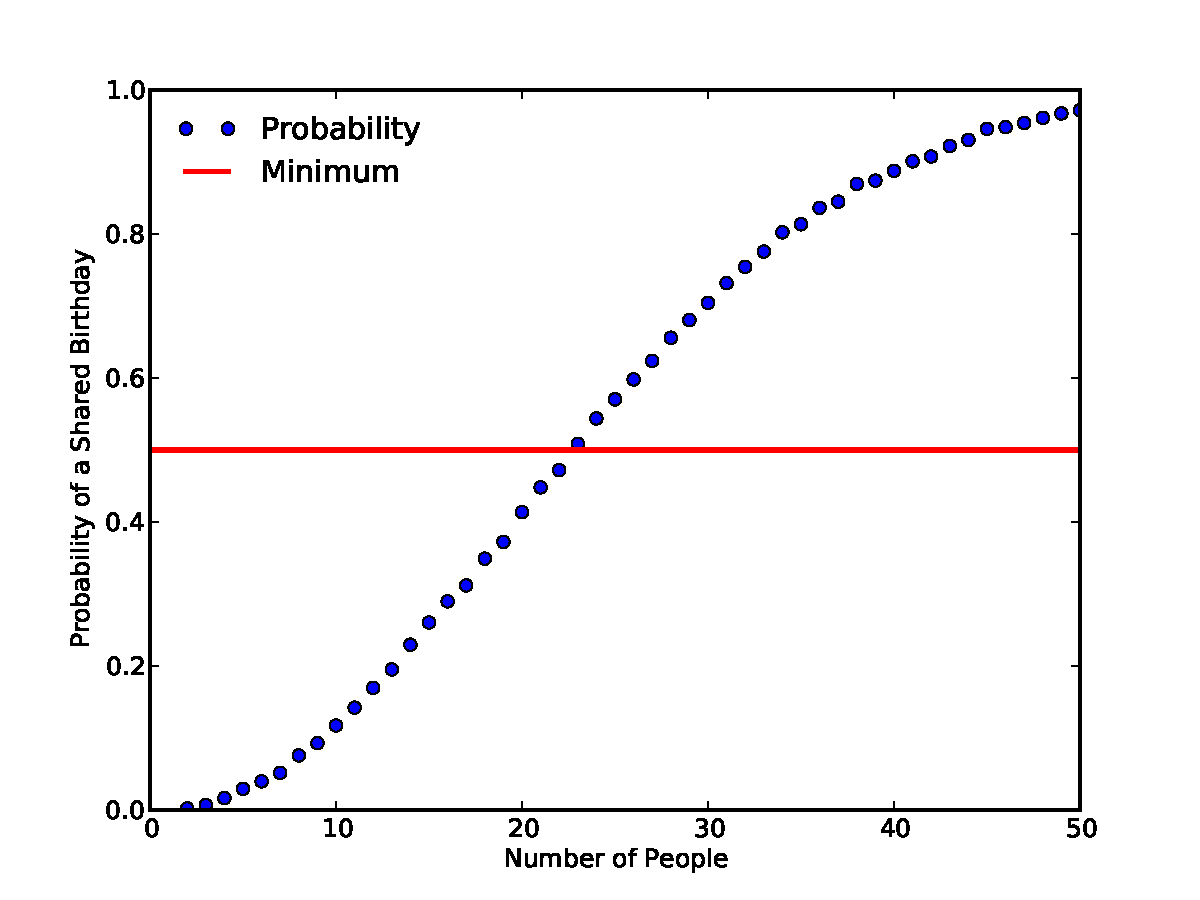
\includegraphics[width=1\textwidth]{Birthday}
  \caption{A plot of the probability of two people in a group having the same birthday vs group size. The first point above the red .5-probability line is 23.}
  \end{figure}

Knowing that 23 people is the minimum, let's check for convergence. Below is a table of calculations of the probability at 23 people for various values of $N$. $N=10$ is off by a significant amount, but it converges to within a few percent for $N \ge 10000$.

\[
\begin{array}{ccc}
\text{Probability} & \text{Fraction} & N \\
0.59999999999999998 & 0.83333333333333337 & 10 \\
0.57999999999999996 & 0.86206896551724144 & 100 \\
0.51400000000000001 & 0.97276264591439687 & 1000 \\
0.50239999999999996 & 0.99522292993630579 & 10000 \\
0.50643000000000005 & 0.98730327982149546 & 100000 \\
0.50710200000000005 & 0.9859949280420901 & 1000000
\end{array}
\]

\section*{Problem 3}

The analytical solution is $22/3 \approx 7.333$. The simulation gets within a percent of this for $N \ge 1000$. It appears to be able to get arbitrarily close as $N$ increases.

\[
\begin{array}{ccc}
\text{Value} & \text{Fraction} & N \\
8.0 & 0.91666666666666663 & 10 \\
7.25 & 1.0114942528735631 & 100 \\
7.4049999999999994 & 0.99032185460274591 & 1000 \\
7.3079999999999998 & 1.0034665207079001 & 10000 \\
7.3167 & 1.0022733381624684 & 100000 \\
7.3371550000000001 & 0.999479135078015 & 1000000
\end{array}
\]


\end{document}









